\section{Vehicle Models} \label{sec:vehicle_models}

A vehicle model defines the position and orientation of a vehicle in the real world and predicts how these states evolve over time.
The choice of model significantly impacts the accuracy and computational complexity of motion planning.
Simpler models, while computationally efficient, may lack precision, whereas more complex models provide higher fidelity but require greater
computational resources.

This section introduces two fundamental models used in trajectory planning [15]: the point mass model, which provides a simplified kinematic
representation, and the bicycle model, which captures essential vehicle dynamics.
In both models, the system's state is represented by a vector $x$, containing relevant variables such as position, velocity, and orientation, while
the control inputs, represented by a vector $u$, influence state transitions over time.
The vehicle dynamics for both models can be generally expressed as:
\begin{equation}
	\dot{x} = f(x, u)
\end{equation}
where $f(x, u)$ represents the system dynamics as a function of the state vector $x$ and the
control inputs $u$.

\subsection{Point Mass Model} \label{subsec:point_mass_model}

The point mass model (PM) represents the vehicle as a point in space with velocity components along the x- and y-axes.
It simplifies vehicle motion by ignoring orientation and steering dynamics, making it computationally efficient for trajectory optimization.
The vehicle state is represented by four variables:

\begin{equation}
	x = \begin{bmatrix} p_x \\ p_y \\ v_x \\ v_y \end{bmatrix}
	\label{eq:states_pm}
\end{equation}
where $p_x$ and $p_y$ define the position in a fixed global coordinate system, while $v_x$ and $v_y$
represent the velocity components in the respective directions.

The control inputs are:

\begin{equation}
	u = \begin{bmatrix} a_x \\ a_y \end{bmatrix}
	\label{eq:controls_pm}
\end{equation}
where $a_x$ and $a_y$ denote accelerations along the $x$- and $y$-axes.
The system follows the linear dynamics:

\begin{equation}
	\dot{x} = \begin{bmatrix}
		v_x \\
		v_y \\
		a_x \\
		a_y
	\end{bmatrix}
\end{equation}

Additionally, the control inputs are constrained by:

\begin{equation}
	\sqrt{u_1^2 + u_2^2} \leq a_{\max}
\end{equation}
where $a_max$ limits the maximum allowable acceleration.
Despite its simplicity, the point mass model is widely used for trajectory planning due to its convex formulation and computational efficiency.
However, it lacks the ability to represent steering dynamics and vehicle orientation, making it less suitable for applications requiring
high-precision maneuvering.

\subsection{Bicycle Model} \label{subsec:bicycle_model}

The bicycle model, also known as the kinematic single-track model (KST), provides a more detailed representation of vehicle motion by incorporating
orientation and steering dynamics.
This model is well-suited for trajectory planning in autonomous driving as it captures essential vehicle behavior while remaining computationally
tractable.

The state vector consists of five variables:
\begin{equation}
	x = \begin{bmatrix} p_x \\ p_y \\ \delta \\ v \\ \psi \end{bmatrix}
	\label{eq:states_kst}
\end{equation}
where:
\begin{itemize}
	\item $p_x$ and $p_y$ represent the vehicle's position in the global coordinate system,
	\item $\delta$ is the front-wheel steering angle,
	\item $v$ is the longitudinal velocity of the rear wheel, and
	\item $\psi$ is the vehicle's orientation relative to the global $x$-axis.
\end{itemize}

The control inputs are:
\begin{equation}
	u = \begin{bmatrix} v_{\delta} \\ a_{x} \end{bmatrix}
	\label{eq:controls_kst}
\end{equation}
where $v_{\delta}$ is the steering velocity, and $a_{\text{long}}$ is the longitudinal acceleration.

The vehicle's motion follows the kinematic equations:
\begin{align}
	 & \dot{p}_x = v\cos(\psi)                                                   \\
	 & \dot{p}_y = v\sin(\psi)                                                   \\
	 & \dot{\delta} = v_{\delta}                                                 \\
	 & \dot{v} = a_{\text{long}}                                                 \\
	 & \dot{\psi} = \frac{v}{l_{wb}} \tan(\delta) \label{eq:dpsi_steering_angle} \\
\end{align}
where $l_wb$ represents the wheelbase length.

The single-track name arises from approximating both front and rear wheels as single contact points, assuming no lateral slip.
This simplification makes the model suitable for path planning while still capturing fundamental steering dynamics.

The bicycle model is visualized in Figure \ref{fig:bicycle_model}.

\begin{figure}[h]
	\centering
	\begin{tikzpicture}
		% Axes
		\draw[->] (0,0) -- (2,0) node[right] {$x$};
		\draw[->] (0,0) -- (0,2) node[above] {$y$};

		% Rear Wheel
		\fill (2,2) circle (2pt); % Draws a small point at (2,2)

		% Vehicle body
		\draw[thick,rotate around={11.536959-90:(2,2)}] (1.8,1.3) rectangle (2.2,2.7);
		\draw[thick,rotate around={26.536959-90:(7,3)}] (6.8,2.3) rectangle (7.2,3.7);

		% Wheelbase
		\draw[-] (2,2) -- (7,3);
		\draw[dashed] (2,2) -- (1.7,3.5);
		\draw[dashed] (7,3) -- (6.7,4.5);
		\draw[dashed, <->] (1.8,3) -- (6.8,4) node[midway,above] {$l_{wb}$};

		% Velocity vector
		\draw[->] (2,2.1) -- (4,2.5) node[midway,above] {$v$};

		% Heading angle
		\draw[dashed] (3.25,2.25) -- (6,2.25);
		\draw[->] (6,2.25) arc (0:11.536959:2.75);
		\node at (5.7,2.5) {$\psi$};

		% Steering angle
		\draw[dashed] (7,3) -- (8.5,3.3);
		\draw[dashed] (7,3) -- ++(26.536959:1.5);
		\draw[->] (8.5,3.3) arc (11.536959:26.536959:1.5);
		\node at (8.2,3.43) {$\delta$};

		% Displacement vector
		\draw[dashed,thick,->] (0,0) -- (1.95,1.95)
		node[midway, left, shift={(-0,+0.4)}] {$\begin{bmatrix}s_x \\ s_y \end{bmatrix}$};
	\end{tikzpicture}
	\caption{Bicycle model representation of a vehicle.}
	\label{fig:bicycle_model}
\end{figure}

Additional constraints ensure realistic vehicle behavior.
A maximum acceleration
constraint is imposed:
\begin{equation}
	\sqrt{u_2^2 + (x_4\dot{x}_5)^2} \leq a_{\max}
\end{equation}

For both models, the vehicle is additionally constrained by its velocity range, steering angle range, and the rate of change of the steering angle.
These constraints are natural and should not be overlooked.

\subsection{Curve Following Coordinate System} \label{subsec:curve_following_coordinate_system}

In addition to the global coordinate system, a curve-following coordinate system, commonly known as the Frenet frame, can be used to simplify the
representation of vehicle motion along a predefined path.
The Frenet frame consists of the arc-length coordinate s and the lateral offset n from the path, as shown in Figure \ref{fig:frenet_frame}.

\begin{figure}[h]
	\centering
	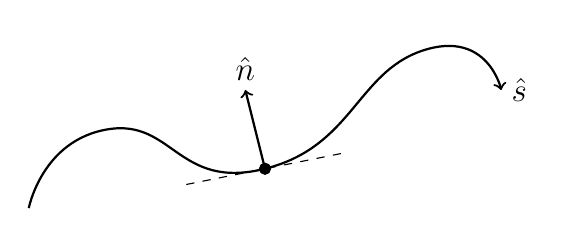
\begin{tikzpicture}
		% Draw the reference path (curved)
		\draw[thick, ->] plot [smooth, tension=1] coordinates {(-3,-1) (-2,0) (0,-0.5) (2,1) (3,0.5)}  node[right] {\large $\hat{s}$};

		% Vehicle position
		\filldraw [black] (0,-0.5) circle (2pt);
		% \node[below left] at (0,-0.5) {\textbf{Vehicle}};

		% Tangent vector (s direction)
		% \draw[->, thick] (0,-0.5) -- (1,0.8);
		% \node[right] at (1,0.8) {\large $\hat{s}$};

		% Normal vector (n direction)
		\draw[->, thick] (0,-0.5) -- (-0.25,0.5);
		\node[above] at (-0.25,0.5) {\large $\hat{n}$};

		% Dashed line for local reference
		\draw[dashed] (-1,-0.7) -- (1,-0.3);
	\end{tikzpicture}
	\caption{Frenet Frame Representation}
	\label{fig:frenet_frame}
\end{figure}